\chapter{Introduction}

With new companies jumping into the Internet of Things (IoT), 
major \emph{IT actors} investing in the development of new
products~\cite{fortuneiot2019}, and telecoms operator building infrastructure 
for the growing demand\footnote{\url{https://www.proximus.be/en/id_cl_iot/companies-and-public-sector/it-services/iot/internet-of-things.html}}.
IoT caught the attention of many people and researcher in the last years.
IoT technology allows the gathering of data and the control of actuators via
the Internet without any human interaction.
The field has been developed during the last decade and has maintained a
consistent growth since.
Business analysts agree that we can expect to reach at least 40 billion
installed \emph{IoT} devices by 2027~\cite{businessinsider2020}.
We are already familiar with the traditional \emph{IoT} products
we use in our households. Those products allow us to connect our light bulbs,
fridge, and washing machine to the Internet.
Meanwhile, we have less knowledge of the industrial usage of \emph{IoT}, also
known as industrial IoT (IIoT). \emph{IIoT} is one of the fastest-growing
segments of the market.
More and more industries are adopting IIoT to consolidate their productions
with \emph{real-time monitoring}, to organize predictive maintenance on their
assets and products to connect their supply chains, etc \ldots

All of this is enabled with the help of sensor networks, and actuators, in a
wide variety of sectors like \emph{smart farming}, \emph{smart cars},
\emph{smart cities}, \emph{energy management}, \ldots

\paragraph{}

All these applications have in common that they rely on devices that
communicate wirelessly.
% TODO Change not telecom
A number of businesses created new technologies to suit this new domain 
that can be classified by three different characteristics

\begin{itemize}
    \item Long or Short \emph{range}
    \item High or low \emph{data-rate}
    \item Low or high \emph{power usage} 
\end{itemize}

% From these characteristics you can only chose two according to the physical
% law. % TODO Explanation needed with the exact law reference explaining this
Figure~\ref{fig:commrangegraph} shows the classification
of the existing wireless communication protocol used in the \emph{IoT} and
presents it in three main categories.

\begin{itemize}
    \item \emph{Short-Range wireless} communication Short-range, high data-rate
    \item \emph{Cellular} communication Long-range, high data-rate
    \item \emph{Low-power wide-area network (LPWAN)} communication Long range,
        low power, and low data-rate
\end{itemize}

\begin{figure}[H] % TODO More info on axis
\centering
\begin{tikzpicture}
    \draw[->,thick] (-0.1,0)--(12,0) node[right]{Range};
    \draw[->,thick] (0,-0.1)--(0,8) node[above]{Data Rate};
    \node[] at (1, -0.5) {10m};
    \draw[] (1,-0.1)--(1,0.1);
    \node[] at (3, -0.5) {100m};
    \draw[] (3,-0.1)--(3,0.1);
    \node[] at (5, -0.5) {1km};
    \draw[] (5,-0.1)--(5,0.1);
    \node[] at (7, -0.5) {10km};
    \draw[] (7,-0.1)--(7,0.1);
    \node[] at (9, -0.5) {100km};
    \draw[] (9,-0.1)--(9,0.1);

    \node[] at (-1.2, 1) {1 kbit/sec};
    \draw[] (-0.1,1)--(0.1,1);
    \node[] at (-1.2, 3) {1 Mbit/sec};
    \draw[] (-0.1,3)--(0.1,3);
    \node[] at (-1.2, 5) {100 Mbit/sec};
    \draw[] (-0.1,5)--(0.1,5);
    \node[] at (-1.2, 7) {1 Gbit/sec};
    \draw[] (-0.1,7)--(0.1,7);
    
    \node[draw] at (8,1.5) (lora) {LoRa};
    \node[draw] at (9.0,0.8) (sigfox) {SigFox};
    \node[draw] at (7.4,2.2) (nb) {NB-IOT};
    \node[draw,dotted,fit=(lora) (sigfox) (nb), label=above:{LPWAN}] {};

    
    \node[draw] at (2.2,3.5) (bluetooth) {Bluetooth};
    \node[draw] at (2.7,2.5) (zigbee) {ZigBee};
    \node[draw] at (2.0,1.8) (ble) {BLE};
    \node[draw] at (3,5) (wifi) {WiFi};
    \node[draw,dotted,fit=(bluetooth) (zigbee) (ble) (wifi), label=above:{Short-range}] {};

    \node[draw] at (6.8,5) (lte) {LTE};
    \node[draw] at (5.8,6) (5g) {5G};
    \node[draw,dotted,fit=(lte) (5g), label=above:{Cellular}] {};
\end{tikzpicture}
\caption{Comparison of the existing IoT wireless technologies by range and data rate}
\label{fig:commrangegraph}
\end{figure}


This work focuses only on \emph{LoRa}, a proprietary \emph{chirp spread spectrum}
modulation technique owned by \emph{Semtech}, operating in the sub-GHz
unlicensed \emph{ISM} band\footnote{Semtech also offers a version of LoRa that
operates in the 2.4GHz band but won't be covered in this text.}. I will cover LoRa 
in more detail in Section~\ref{section:lora}.
The main characteristics of \emph{LoRa} are its low power transmission and the
fact that it can trade throughput for range by fine-tuning the physical layer
(PHY) settings.
The long-range capabilities of the protocol caught the attention of
many people. 
Some have succeeded in obtaining a record transmission distance of over 700 km with
a direct line of sight between the receiver and the
transmitter~\cite{network_2017}.
However, this case is not a real-world example. The range in urban areas is
around \emph{2 to 5 km} and around \emph{15 km} in suburban
areas~\cite{8030482}.

\emph{LoRa} is often used in conjunction with \emph{LoRaWAN}, an ALOHA 
based~\cite{loraalliance:lorawanspecification} MAC protocol deployed in a star-of-stars 
topology.
LoRaWAN is composed of wireless \emph{motes} sending messages to \emph{gateways} (GWs).
Those GWs are connected to the internet and will relay messages to central servers
as we can see in Figure~\ref{fig:startopology}.
This single-hop topology has been successful because free (as well as paid
services) LoRaWAN network to connect to already exists
\footnote{\url{https://www.thethingsnetwork.org/map}} and free private networks are
deployable in contrast to other LPWAN like \emph{Sigfox} or \emph{NB-IoT}.

\begin{figure}[H]
\begin{subfigure}[b]{.5\textwidth}
    \centering
    \begin{tikzpicture}[auto, thick]
      % Place super peers and connect them
      \foreach \place/\name in {{(0,-1)/a}, {(2,0)/b}, {(2.5, -3)/c}}
        \node[gateways] (\name) at \place {};
      \node[server] (d) at (1.5,-1.5) {};
      %
      \foreach \source/\dest in {a/d, b/d}
        \path[dotted] (\source) edge (\dest);
      \path (c) edge (d); % Non dotted
      %
      % Place normal peers
      \foreach \pos/\i in {above right of/1, right of/2, below right of/3}
        \node[motes, \pos =b ] (b\i) {};
      \foreach \speer/\peer in {b/b1,b/b2,b/b3}
        \path[dotted] (\speer) edge (\peer);
      %
      \foreach \pos/\i in {below left of/1, below of/2, left of/3, above right of/4}
        \node[motes, \pos =a ] (a\i) {};
      \foreach \speer/\peer in {a/a1,a/a2,a/a3,a/a4}
        \path[dotted] (\speer) edge (\peer);
      %
      \path[dotted] (b) edge (a4);
    \end{tikzpicture}
    \caption{Star topology}
    \label{fig:startopology}
\end{subfigure}
\hfill
\begin{subfigure}[b]{.5\textwidth}
    \centering
    \begin{tikzpicture}[auto, thick]
      % Place super peers and connect them
      \foreach \place/\name in {{(0,-1)/a}, {(2,0)/b}, {(2, -3)/c}, {(1,1)/d}, {(1.5, -1.5)/f}}
        \node[motes] (\name) at \place {};
      \foreach \source/\dest in {a/b, a/c, b/c, d/b, f/a, f/b, f/c}
        \path[dotted] (\source) edge (\dest);
      %
      % Place normal peers
      \foreach \pos/\i in {above right of/1, right of/2, below right of/3}
        \node[motes, \pos =b ] (b\i) {};
      \foreach \speer/\peer in {b/b1,b/b2,b/b3}
        \path[dotted] (\speer) edge (\peer);
      %
      \foreach \pos/\i in {above left of/1, left of/2, above of/3}
        \node[motes, \pos =d ] (d\i) {};
      \foreach \speer/\peer in {d/d1,d/d2,d/d3}
        \path[dotted] (\speer) edge (\peer);
      %
      \foreach \pos/\i in {below left of/1, below of/2, left of/3}
        \node[motes, \pos =a ] (a\i) {};
      \foreach \speer/\peer in {a/a1,a/a2,a/a3}
        \path[dotted] (\speer) edge (\peer);
    \end{tikzpicture}
    \caption{Mesh Network Topology}
    \label{fig:meshtopology}
\end{subfigure}
\caption{Different LoRa Network Topologies}
\label{fig:topologies}
\end{figure}




The issue with \emph{LoRaWAN}, as studied 
in~\cite{8030482}~\cite{10.1145/2988287.2989163} is its inability to scale. 

Channel sensing is impossible in LoRa because \emph{Channel Activity Detection}
(CAD) only detects the packet preamble. % TODO reference needed
This leads to collision when motes transmit at the same time.
On collision, the transmission has to be re-done using a back-off strategy till the
message has been correctly received or the number of trials has reached its
maximum.
This implies a higher energy consumption for the motes and more radio 
channel usage.
As the network gets denser~\cite{8030482}, the effect of collisions gets
increasingly significant with little to no packets received by gateways.

% TODO Figure from the paper about received packets ?

The \emph{duty-cycle} regulations in place for the \emph{ISM} bands on every
transmitting device (motes and gateways) is also a limiting factor 
for \emph{LoRaWAN} (\cite{8030482}).
The European ISM band has set a duty-cycle of \emph{1\%} meaning that each node 
and gateway can transmit \emph{36 sec/hour} maximum. 

% TODO {Add some reference to ISM regulations} 

Link quality also influences LoRaWAN's efficiency. 
Environmental factors like temperature,
humidity~\cite{evaluation_of_the_reliability_of_lora}, and the topology of the
terrain~\cite{lorajambalaya}, influence the link quality.
All these factors make network coverage typically not uniform 
as in Fig~\ref{fig:coverage}.
Motes on the border of the gateway coverage area may struggle to
achieve a full transmission. 

Gateways could restrain the deployment of LoRa networks.
They might not be deployed everywhere as they require more demanding infrastructure 
than battery-operated motes.
That is the case for pipelines and tunnels~\cite{Abrardo_2019},
we would prefer to only install motes running on batteries as in linear
topology gateways are not of any use.
They can also be a single point of failure of the network, when a single
gateway covers a portion of the network. 

\begin{figure}[H]
    \centering
    \def\angle{0}
    \def\radius{3}
    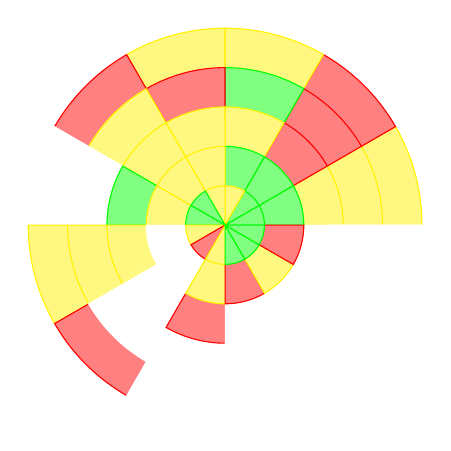
\begin{tikzpicture}[nodes = {font=\sffamily}]
      \foreach \color in {
            yellow,
            red,
            yellow,
            white,
            red,
            yellow,
            white,
            yellow,
            white,
            white,
            red,
            red,
        } {
        \ifx\color\empty\else
            \draw[fill={\color!50},draw={\color}] (0,0) -- (\angle:\radius)
              arc (\angle:\angle+30:\radius) -- cycle;
            \pgfmathparse{\angle+30}
            \xdef\angle{\pgfmathresult}
        \fi
        };
        \xdef\radius{2.5}
        \foreach \color in {
            yellow,
            red,
            yellow,
            yellow,
            red,
            white,
            yellow,
            red,
            white,
            white,
            white,
            white,
        } {
        \ifx\color\empty\else
            \draw[fill={\color!50},draw={\color}] (0,0) -- (\angle:\radius)
              arc (\angle:\angle+30:\radius) -- cycle;
            \pgfmathparse{\angle+30}
            \xdef\angle{\pgfmathresult}
        \fi
        };
        \xdef\radius{2}
        \foreach \color in {
            yellow,
            red,
            green,
            red,
            yellow,
            white,
            yellow,
            white,
            white,
            white,
            white,
            white,
        } {
        \ifx\color\empty\else
            \draw[fill={\color!50},draw={\color}] (0,0) -- (\angle:\radius)
              arc (\angle:\angle+30:\radius) -- cycle;
            \pgfmathparse{\angle+30}
            \xdef\angle{\pgfmathresult}
        \fi
        };
        \xdef\radius{1.5}
        \foreach \color in {
            yellow,
            red,
            yellow,
            yellow,
            yellow,
            green,
            yellow,
            white,
            red,
            white,
            white,
            white,
        } {
        \ifx\color\empty\else
            \draw[fill={\color!50},draw={\color}] (0,0) -- (\angle:\radius)
              arc (\angle:\angle+30:\radius) -- cycle;
            \pgfmathparse{\angle+30}
            \xdef\angle{\pgfmathresult}
        \fi
        };
        \xdef\radius{1}
        \foreach \color in {
            green,
            green,
            green,
            yellow,
            yellow,
            yellow,
            white,
            white,
            yellow,
            red,
            yellow,
            red,
        } {
        \ifx\color\empty\else
            \draw[fill={\color!50},draw={\color}] (0,0) -- (\angle:\radius)
              arc (\angle:\angle+30:\radius) -- cycle;
            \pgfmathparse{\angle+30}
            \xdef\angle{\pgfmathresult}
        \fi
        };
        \xdef\radius{0.5}
        \foreach \color in {
            green,
            green,
            yellow,
            yellow,
            green,
            green,
            yellow,
            red,
            yellow,
            green,
            green,
            green,
        } {
        \ifx\color\empty\else
            \draw[fill={\color!50},draw={\color}] (0,0) -- (\angle:\radius)
              arc (\angle:\angle+30:\radius) -- cycle;
            \pgfmathparse{\angle+30}
            \xdef\angle{\pgfmathresult}
        \fi
        };
    \end{tikzpicture}
\caption{Typical gateway coverage\cite{lorajambalaya}}
\label{fig:coverage}

\begin{tabular}{r@{: }l r@{: }l}

\begin{tikzpicture}\draw[fill=green,line width=1pt]  circle(1ex);\end{tikzpicture} & Good\ Connection & 
\begin{tikzpicture}\draw[fill=yellow,line width=1pt]  circle(1ex);\end{tikzpicture} & Intermediate\ Connection\\

\begin{tikzpicture}\draw[fill=red,line width=1pt]  circle(1ex);\end{tikzpicture} & Bad\ Connection & 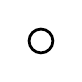
\begin{tikzpicture}\draw[fill=white,line width=1pt]  circle(1ex);\end{tikzpicture} & No\ Connection 
\end{tabular}
\end{figure}




Multi-hop networks, as represented in Figure~\ref{fig:meshtopology}, can be a solution to
the LoRaWAN scaling issues~\cite{8115756}.
Participants of the network do not directly send message to gateways, but
instead, pass messages to their neighboring nodes.
Using a multi-hop routing protocol increases the reliability, the range
and can adapt to topology changes in the network (because of moving or failing nodes).

Multi-hop routing protocols are de facto a strong candidate for large area monitoring 
applications where gateways may be hard and costly to deploy and where blind
spots often arise.
This solution can decrease the energy consumption of bordering nodes that
usually struggle to achieve successful communication on non-optimal
conditions.

\paragraph{}

Work to create a multi-hop routing protocol with LoRa has already been
done~\cite{8115756, DIAS2018424, 8856256, Abrardo_2019, duong2018}, 
but some of them did not take into account the energy consumption of the nodes
with always-on radio to listen to incoming communication.
This is completely contrary to the benefit of using LPWAN networks typically
based on sleeping nodes.

A solution to this matter would be to use time-slotted channel access.
It would suppress collisions and schedule communications between nodes leaving
the nodes in a sleeping state the rest of the time.

The \emph{IEEE 802.15.4e} standard developed TSCH, a MAC
protocol to use with 802.15.4 compliant physical layer.
TSCH works particularly well where LoRaWAN shows weaknesses. 
TSCH is resilient to external interference with the use of channel hopping.
Networks with high node density can work without collision issues.
It also provides high reliability communications and deterministic delays by 
keeping the nodes time-synchronized.

\paragraph{}

This thesis aims to adapt the TSCH MAC protocol for LoRa,
thus bringing a reliable, long-range and low power IPv6 multi-hop
solution to the LoRa ecosystem.

Work to adapt TSCH for LoRa in~\cite{8847137} and~\cite{njomgang_2018}, has
already been done in the previous year at \emph{VUB}.
This thesis builds on the combined efforts of the previous
years to adapt \emph{TSCH} for the \emph{Zolertia RE-Mote} and the
\emph{RN2483} LoRa shield.

\paragraph{}

Chapter \ref{section:context} will give the background information and context needed to
understand the building blocks to achieve my end goal.
It will also give an overview of the related work on the subject of
LoRa multi-hop communications.
Chapter 3 gives the implementation details of writing a driver for the
RN2483 in Contiki OS and the experimentation with the driver.
Chapter 4 gives instructions for adapting and operating TSCH with LoRa on
Contiki OS as well as the different testing I conducted.
Finally, Chapter 5 will conclude the work by summarizing it and suggesting
further research possible on the subject.
